\documentclass[11pt,a4paper]{report}
\usepackage[textwidth=37em,vmargin=30mm]{geometry}
\usepackage{calc,xunicode,amsmath,amssymb,paralist,enumitem,tabu,booktabs,datetime2,xeCJK,xeCJKfntef,listings}
\usepackage{tocloft,fancyhdr,tcolorbox,xcolor,graphicx,eso-pic,xltxtra,xelatexemoji}

\newcommand{\envyear}[0]{2025}
\newcommand{\envdatestr}[0]{2025-03-25}
\newcommand{\envfinaldir}[0]{webdb/2025/20250325/final}

\usepackage[hidelinks]{hyperref}
\hypersetup{
    colorlinks=false,
    pdfpagemode=FullScreen,
    pdftitle={Web Digest - \envdatestr}
}

\setlength{\cftbeforechapskip}{10pt}
\renewcommand{\cftchapfont}{\rmfamily\bfseries\large\raggedright}
\setlength{\cftbeforesecskip}{2pt}
\renewcommand{\cftsecfont}{\sffamily\small\raggedright}

\setdefaultleftmargin{2em}{2em}{1em}{1em}{1em}{1em}

\usepackage{xeCJK,xeCJKfntef}
\xeCJKsetup{PunctStyle=plain,RubberPunctSkip=false,CJKglue=\strut\hskip 0pt plus 0.1em minus 0.05em,CJKecglue=\strut\hskip 0.22em plus 0.2em}
\XeTeXlinebreaklocale "zh"
\XeTeXlinebreakskip = 0pt


\setmainfont{Brygada 1918}
\setromanfont{Brygada 1918}
\setsansfont{IBM Plex Sans}
\setmonofont{JetBrains Mono NL}
\setCJKmainfont{Noto Serif CJK SC}
\setCJKromanfont{Noto Serif CJK SC}
\setCJKsansfont{Noto Sans CJK SC}
\setCJKmonofont{Noto Sans CJK SC}

\setlength{\parindent}{0pt}
\setlength{\parskip}{8pt}
\linespread{1.15}

\lstset{
	basicstyle=\ttfamily\footnotesize,
	numbersep=5pt,
	backgroundcolor=\color{black!5},
	showspaces=false,
	showstringspaces=false,
	showtabs=false,
	tabsize=2,
	captionpos=b,
	breaklines=true,
	breakatwhitespace=true,
	breakautoindent=true,
	linewidth=\textwidth
}






\newcommand{\coverpic}[2]{
    % argv: itemurl, authorname
    Cover photo by #2~~(\href{#1}{#1})
}
\newcommand{\makeheader}[0]{
    \begin{titlepage}
        % \newgeometry{hmargin=15mm,tmargin=21mm,bmargin=12mm}
        \begin{center}
            
            \rmfamily\scshape
            \fontspec{BaskervilleF}
            \fontspec{Old Standard}
            \fontsize{59pt}{70pt}\selectfont
            WEB\hfill DIGEST
            
            \vfill
            % \vskip 30pt
            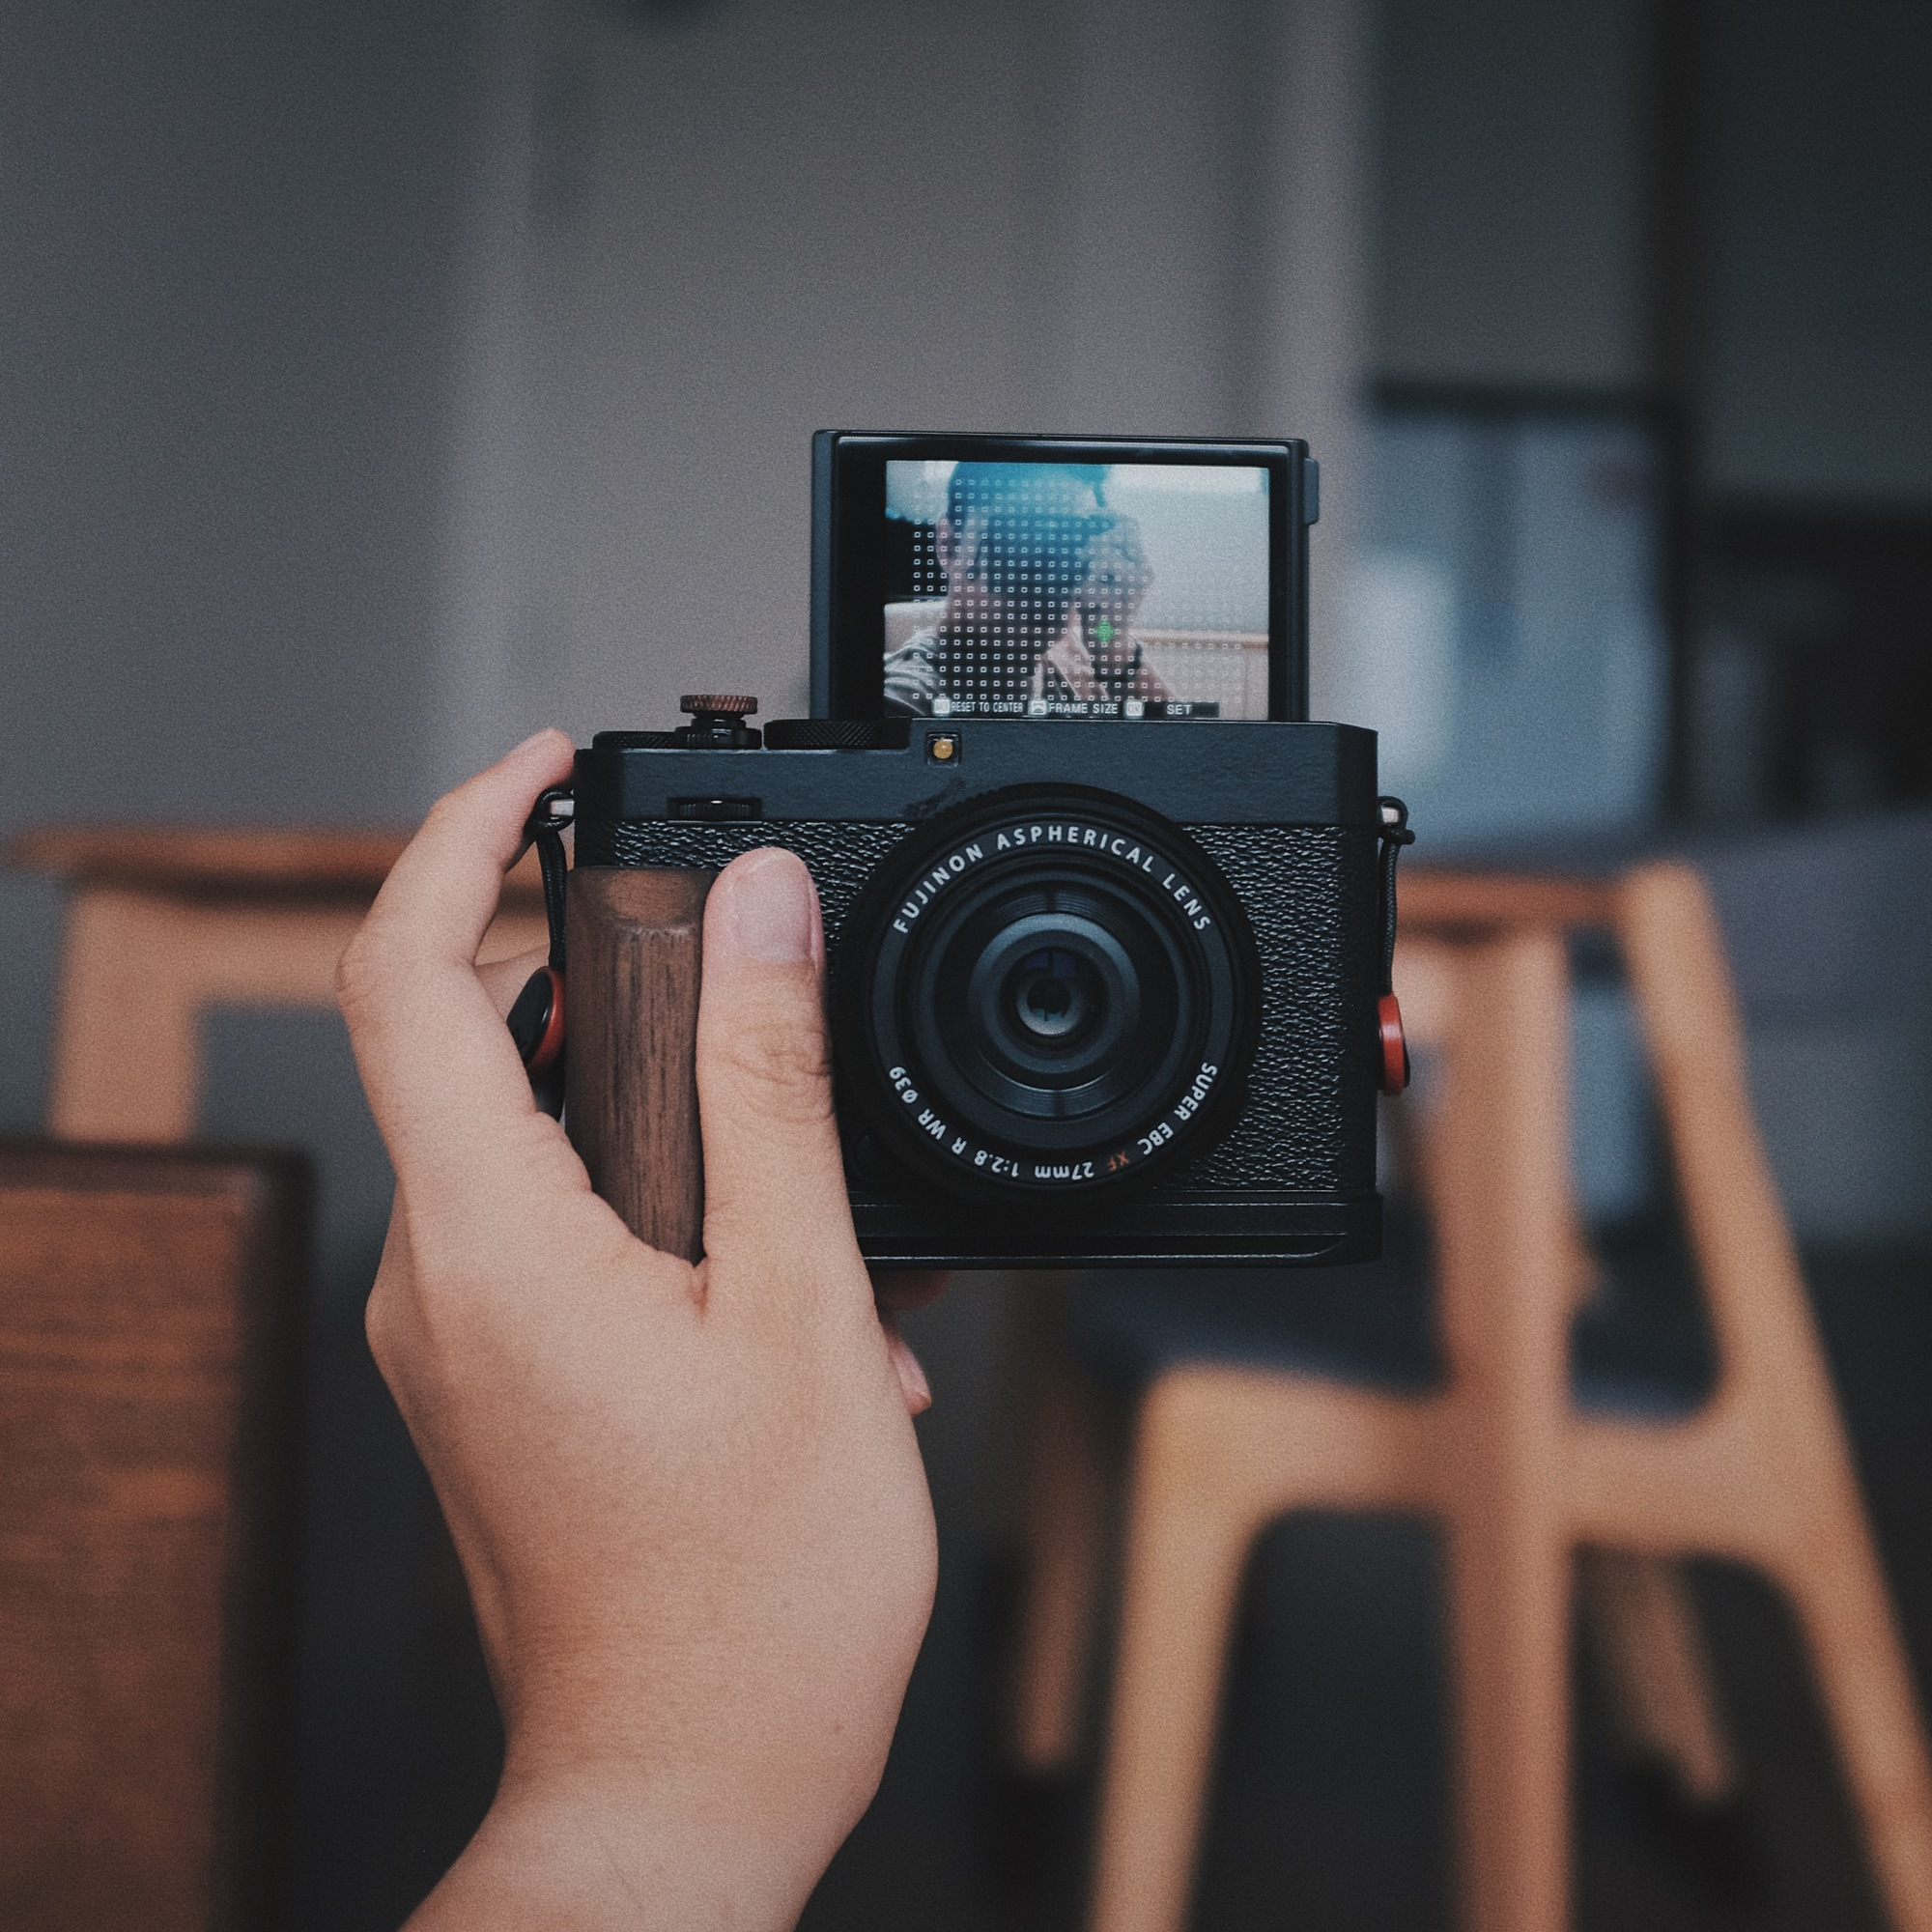
\includegraphics[width=\linewidth]{\envfinaldir/coverpic-prod.jpg}\par
            % \vskip 30pt
            \vfill

            \normalsize\rmfamily\scshape
            \copyright{} The Web Digest Project \hfill\large \envdatestr
        \end{center}
    \end{titlepage}
    % \restoregeometry
}
\newcommand{\simplehref}[1]{%
    \textcolor{blue!80!green}{\href{#1}{#1}}%
}
\renewcommand{\contentsname}{\center\Huge\sffamily\bfseries Contents\par\vskip 20pt}
\newcounter{ipartcounter}
\setcounter{ipartcounter}{0}
\newcommand{\ipart}[1]{
    % \vskip 20pt
    \clearpage
    \stepcounter{ipartcounter}
    \phantomsection
    \addcontentsline{toc}{chapter}{#1}
    % \begin{center}
    %     \Huge
    %     \sffamily\bfseries
    %     #1
    % \end{center}
    % \vskip 20pt plus 7pt
}
\newcounter{ichaptercounter}
\setcounter{ichaptercounter}{0}
\newcommand{\ichapter}[1]{
    % \vskip 20pt
    \clearpage
    \stepcounter{ichaptercounter}
    \phantomsection
    \addcontentsline{toc}{section}{\numberline{\arabic{ichaptercounter}}#1}
    \begin{center}
        \Huge
        \sffamily\bfseries
        #1
    \end{center}
    \vskip 20pt plus 7pt
}
\newcommand{\entrytitlefont}[1]{\subsection*{\raggedright\Large\sffamily\bfseries#1}}
\newcommand{\entryitemGeneric}[2]{
    % argv: title, url
    \parbox{\linewidth}{
        \entrytitlefont{#1}\par\vskip 5pt
        \footnotesize\ttfamily\mdseries
        \simplehref{#2}
    }\vskip 11pt plus 11pt minus 1pt
}
\newcommand{\entryitemGithub}[3]{
    % argv: title, url, desc
    \parbox{\linewidth}{
        \entrytitlefont{#1}\par\vskip 5pt
        \footnotesize\ttfamily\mdseries
        \simplehref{#2}\par\vskip 5pt
        \small\rmfamily\mdseries#3
    }\vskip 11pt plus 11pt minus 1pt
}
\newcommand{\entryitemAp}[3]{
    % argv: title, url, desc
    \parbox{\linewidth}{
        \entrytitlefont{#1}\par\vskip 5pt
        \footnotesize\ttfamily\mdseries
        \simplehref{#2}\par\vskip 5pt
        \small\rmfamily\mdseries#3
    }\vskip 11pt plus 11pt minus 1pt
}
\newcommand{\entryitemHackernews}[3]{
    % argv: title, hnurl, rawurl
    % \parbox{\linewidth}{
    %     \entrytitlefont{#1}\par\vskip 5pt
    %     \footnotesize\ttfamily\mdseries
    %     \simplehref{#3}\par
    %     \textcolor{black!50}{\href{#2}{#2}}
    % }\vskip 11pt plus 11pt minus 1pt
    \begin{minipage}{\linewidth}
            \entrytitlefont{#1}\par\vskip 5pt
            \footnotesize\ttfamily\mdseries
            \simplehref{#3}\par
            \textcolor{black!50}{\href{#2}{#2}}
    \end{minipage}\par\vskip 11pt plus 11pt minus 1pt
}







\begin{document}

\makeheader

\tableofcontents\clearpage




\ipart{Developers}
\ichapter{Hacker News}
\entryitemTwoLinks{Internet Archive Europe – Bringing Collections to Life}{https://news.ycombinator.com/item?id=43464230}{https://www.internetarchive.eu/}

\entryitemTwoLinks{Qwen2.5-VL-32B: Smarter and Lighter}{https://news.ycombinator.com/item?id=43464068}{https://qwenlm.github.io/blog/qwen2.5-vl-32b/}

\entryitemTwoLinks{I won't connect my dishwasher to your cloud}{https://news.ycombinator.com/item?id=43463200}{https://www.jeffgeerling.com/blog/2025/i-wont-connect-my-dishwasher-your-stupid-cloud}

\entryitemTwoLinks{The Trump administration accidentally texted me its war plans}{https://news.ycombinator.com/item?id=43462783}{https://www.theatlantic.com/politics/archive/2025/03/trump-administration-accidentally-texted-me-its-war-plans/682151/}

\entryitemTwoLinks{Mastering Delphi 5 2025 Annotated Edition Is Now Complete}{https://news.ycombinator.com/item?id=43462299}{https://blog.marcocantu.com/blog/2025-march-mastering-delphi5-annotated-complete.html}

\entryitemTwoLinks{Triforce – a beamformer for Apple Silicon laptops}{https://news.ycombinator.com/item?id=43461701}{https://crates.io/crates/triforce-lv2}

\entryitemTwoLinks{Goblin.tools: simple, single-task tools to help neurodivergent people with tasks}{https://news.ycombinator.com/item?id=43461375}{https://goblin.tools/}

\entryitemTwoLinks{The game designer playing through his own psyche}{https://news.ycombinator.com/item?id=43459361}{https://www.newyorker.com/culture/persons-of-interest/the-game-designer-playing-through-his-own-psyche}

\entryitemTwoLinks{Japanese scientists use stem cell treatment to restore movement in spinal injury}{https://news.ycombinator.com/item?id=43459264}{https://medicalxpress.com/news/2025-03-japanese-scientists-stem-cell-treatment.html}

\entryitemTwoLinks{HP avoids monetary damages over bricked printers in class-action settlement}{https://news.ycombinator.com/item?id=43458759}{https://arstechnica.com/gadgets/2025/03/hp-avoids-monetary-damages-over-bricked-printers-in-class-action-settlement/}

\entryitemTwoLinks{Tesla sales drop 35\% in San Diego County}{https://news.ycombinator.com/item?id=43458758}{https://fox5sandiego.com/news/business/tesla-sales-drop-35-in-san-diego-county/}

\entryitemTwoLinks{European Cloud, Global Reach}{https://news.ycombinator.com/item?id=43458717}{https://upcloud.com/blog/european-cloud-global-reach}

\entryitemTwoLinks{Millions are visiting the European Alternatives site. What trends are we seeing?}{https://news.ycombinator.com/item?id=43458509}{https://plausible.io/blog/european-alternatives-trends-privacy-tech}

\entryitemTwoLinks{Osgint – OSINT tool to find information about GitHub user}{https://news.ycombinator.com/item?id=43458033}{https://github.com/hippiiee/osgint}

\entryitemTwoLinks{23andMe files for bankruptcy to sell itself}{https://news.ycombinator.com/item?id=43457666}{https://www.reuters.com/business/healthcare-pharmaceuticals/dna-testing-firm-23andme-files-chapter-11-bankruptcy-sell-itself-2025-03-24/}

\entryitemTwoLinks{The Vatican's Latinist (2017)}{https://news.ycombinator.com/item?id=43457202}{https://newcriterion.com/article/the-vaticans-latinist/}

\entryitemTwoLinks{63 Chinese Cuisines: The Complete Guide (2024)}{https://news.ycombinator.com/item?id=43457180}{https://chinesecookingdemystified.substack.com/p/63-chinese-cuisines-the-complete}

\entryitemTwoLinks{Move on to ESM-Only}{https://news.ycombinator.com/item?id=43456966}{https://antfu.me/posts/move-on-to-esm-only}

\entryitemTwoLinks{Quadlet: Running Podman containers under systemd}{https://news.ycombinator.com/item?id=43456934}{https://mo8it.com/blog/quadlet/}

\entryitemTwoLinks{Project Aardvark: reimagining AI weather prediction}{https://news.ycombinator.com/item?id=43456723}{https://www.turing.ac.uk/blog/project-aardvark-reimagining-ai-weather-prediction}\ichapter{Phoronix}
\entryitemGeneric{\hskip 0pt{}GIMP 3.0.2 Released To Fix Early Bugs From GIMP 3.0}{https://www.phoronix.com/news/GIMP-3.0.2-Released}

\entryitemGeneric{\hskip 0pt{}Bcachefs Aims For "Soft Frozen" On-Disk Format With Linux 6.15 Along With New Features}{https://www.phoronix.com/news/Bcachefs-Linux-6.15}

\entryitemGeneric{\hskip 0pt{}Btrfs Adding Fast/Realtime Zstd Compression \& Other Performance Optimizations}{https://www.phoronix.com/news/Linux-6.15-Btrfs}

\entryitemGeneric{\hskip 0pt{}New FWCTL Subsystem Submitted For Linux 6.15}{https://www.phoronix.com/news/Linux-6.15-fwctl}

\entryitemGeneric{\hskip 0pt{}AMD Lands LLVM Flang Fortran Runtime Support For Compiling Directly On The GPU}{https://www.phoronix.com/news/AMD-Flang-RT-Build-On-GPU}

\entryitemGeneric{\hskip 0pt{}Linux 6.14 Released With Working NTSYNC Driver, AMD Ryzen AI Accelerator Support}{https://www.phoronix.com/news/Linux-6.14}

\entryitemGeneric{\hskip 0pt{}Intel's AVX10.2 Patches Merged For GCC 15 To Drop 256-bit Rounding \& AVX10.2-256 Options}{https://www.phoronix.com/news/Intel-AVX10.2-256-Merged-GCC-15}

\entryitemGeneric{\hskip 0pt{}Faster Intel/AMD Crypto Performance \& Initial Intel APX Enablement Slated For Linux 6.15}{https://www.phoronix.com/news/Linux-6.15-x86-FPU}

\entryitemGeneric{\hskip 0pt{}Wayland Protocols 1.42 Updates Cursor Shape \& Tablet Protocols}{https://www.phoronix.com/news/Wayland-Protocols-1.42}\ichapter{Dribbble}
\entryitemGeneric{\hskip 0pt{}Aura - Logo Design}{https://dribbble.com/shots/25815819-Aura-Logo-Design}

\entryitemGeneric{\hskip 0pt{}Phantom auto buy/sell concept}{https://dribbble.com/shots/25799751-Phantom-auto-buy-sell-concept}

\entryitemGeneric{\hskip 0pt{}Task completion micro interaction}{https://dribbble.com/shots/25797132-Task-completion-micro-interaction}

\entryitemGeneric{\hskip 0pt{}PurePaws - Logo Design}{https://dribbble.com/shots/25797575-PurePaws-Logo-Design}

\entryitemGeneric{\hskip 0pt{}Central Coast}{https://dribbble.com/shots/25794367-Central-Coast}

\entryitemGeneric{\hskip 0pt{}S mark}{https://dribbble.com/shots/25796446-S-mark}

\entryitemGeneric{\hskip 0pt{}The Sequencer Poster}{https://dribbble.com/shots/25798231-The-Sequencer-Poster}

\entryitemGeneric{\hskip 0pt{}Puzzle Fintech UI/UX design, User Interface experience}{https://dribbble.com/shots/25652036-Puzzle-Fintech-UI-UX-design-User-Interface-experience}

\entryitemGeneric{\hskip 0pt{}Sidebar Navigation for Core 2.0 – Dashboard Builder}{https://dribbble.com/shots/25790810-Sidebar-Navigation-for-Core-2-0-Dashboard-Builder}

\entryitemGeneric{\hskip 0pt{}Novascan}{https://dribbble.com/shots/25790443-Novascan}

\entryitemGeneric{\hskip 0pt{}Plain - Branding}{https://dribbble.com/shots/25790107-Plain-Branding}

\entryitemGeneric{\hskip 0pt{}Decades of Unforgettable Hits}{https://dribbble.com/shots/25792477-Decades-of-Unforgettable-Hits}

\entryitemGeneric{\hskip 0pt{}Mixed Stickers}{https://dribbble.com/shots/25737407-Mixed-Stickers}

\entryitemGeneric{\hskip 0pt{}Halo Movie poster}{https://dribbble.com/shots/25791667-Halo-Movie-poster}

\entryitemGeneric{\hskip 0pt{}Finory app}{https://dribbble.com/shots/25778453-Finory-app}

\entryitemGeneric{\hskip 0pt{}Lemur}{https://dribbble.com/shots/25792165-Lemur}

\entryitemGeneric{\hskip 0pt{}Crypto Bridge}{https://dribbble.com/shots/25783744-Crypto-Bridge}

\entryitemGeneric{\hskip 0pt{}Cargo Shipment App UI}{https://dribbble.com/shots/25784159-Cargo-Shipment-App-UI}

\entryitemGeneric{\hskip 0pt{}Eclipse - Logo Design}{https://dribbble.com/shots/25784396-Eclipse-Logo-Design}

\entryitemGeneric{\hskip 0pt{}Burn Bright, Take Flight}{https://dribbble.com/shots/25778930-Burn-Bright-Take-Flight}

\entryitemGeneric{\hskip 0pt{}Core 2.0 – Dashboard Builder}{https://dribbble.com/shots/25782776-Core-2-0-Dashboard-Builder}

\entryitemGeneric{\hskip 0pt{}The Planner app}{https://dribbble.com/shots/25769751-The-Planner-app}

\entryitemGeneric{\hskip 0pt{}PieLabs Unused Logo Design}{https://dribbble.com/shots/25784372-PieLabs-Unused-Logo-Design}

\entryitemGeneric{\hskip 0pt{}Mammut ID Concept}{https://dribbble.com/shots/25784364-Mammut-ID-Concept}


\ipart{Developers~~~~(zh-Hans)}
\ichapter{Solidot}
\entryitemGeneric{\hskip 0pt{}库克访华,宣布设立 7.2 亿元清洁能源投资基金}{https://www.solidot.org/story?sid=80870}

\entryitemGeneric{\hskip 0pt{}Linux Kernel 6.14 释出}{https://www.solidot.org/story?sid=80869}

\entryitemGeneric{\hskip 0pt{}波音将为美国空军制造下一代隐形战斗机 F-47}{https://www.solidot.org/story?sid=80868}

\entryitemGeneric{\hskip 0pt{}European Alternatives 网站今年至今吸引了逾百万访客}{https://www.solidot.org/story?sid=80866}

\entryitemGeneric{\hskip 0pt{}Facebook 告密者寻求推翻采访禁令}{https://www.solidot.org/story?sid=80865}

\entryitemGeneric{\hskip 0pt{}已知最遥远星系中发现氧元素}{https://www.solidot.org/story?sid=80864}

\entryitemGeneric{\hskip 0pt{}23andMe 申请破产保护}{https://www.solidot.org/story?sid=80863}

\entryitemGeneric{\hskip 0pt{}AI 编程助手能通过规则文件生成后门}{https://www.solidot.org/story?sid=80862}

\entryitemGeneric{\hskip 0pt{}摧毁x86最后堡垒:Intel电熔丝e-Fuse加密密钥泄漏}{https://www.solidot.org/story?sid=80861}

\entryitemGeneric{\hskip 0pt{}前往美国最好带上一次性使用的手机}{https://www.solidot.org/story?sid=80860}

\entryitemGeneric{\hskip 0pt{}匈牙利禁止骄傲游行将利用面部识别技术去识别参与者}{https://www.solidot.org/story?sid=80859}

\entryitemGeneric{\hskip 0pt{}俄测试网络主权,完全切断 Cloudflare 连接}{https://www.solidot.org/story?sid=80858}

\entryitemGeneric{\hskip 0pt{}休闲游戏增加老年人的幸福感}{https://www.solidot.org/story?sid=80857}

\entryitemGeneric{\hskip 0pt{}意大利要求 Google DNS 服务器修改盗版网站的 DNS 解析}{https://www.solidot.org/story?sid=80856}

\entryitemGeneric{\hskip 0pt{}AMD 推出在本地运行大模型的开源项目 Gaia }{https://www.solidot.org/story?sid=80855}

\entryitemGeneric{\hskip 0pt{}微软通过电子邮件建议 Windows 10 用户购买新 PC}{https://www.solidot.org/story?sid=80854}

\entryitemGeneric{\hskip 0pt{}雅虎将 TechCrunch 出售给 Regent}{https://www.solidot.org/story?sid=80853}\ichapter{V2EX}
\entryitemGeneric{\hskip 0pt{}[问与答] 本人大三二本人工智能专业正准备考研, v 友们帮我想个复试有用的毕设}{https://www.v2ex.com/t/1120825}

\entryitemGeneric{\hskip 0pt{}[酷工作] 美国 Biotech Startup 招募前后端工程师}{https://www.v2ex.com/t/1120823}

\entryitemGeneric{\hskip 0pt{}[宽带症候群] 无语了, speedtest.net 竟然被墙了}{https://www.v2ex.com/t/1120822}

\entryitemGeneric{\hskip 0pt{}[程序员] Cursor 等 AI IDE 怎么解决单文件一万行的这种超长上下文?例如我公司有个项目后端所有业务逻辑都在 BusinessService.cs 里,里面分了六十几个 Region, Cursor 完全处理不了这个文件,一直提示网络错误}{https://www.v2ex.com/t/1120821}

\entryitemGeneric{\hskip 0pt{}[问与答] 项目冷启动,咱这里有没有实战经验的盆友啊!}{https://www.v2ex.com/t/1120820}

\entryitemGeneric{\hskip 0pt{}[分享创造] 写了一个支持 MCP 的聊天记录查询小工具(支持 macOS)}{https://www.v2ex.com/t/1120819}

\entryitemGeneric{\hskip 0pt{}[问与答] 听劝大学生该如何选择未来?求助各位 V2er!}{https://www.v2ex.com/t/1120818}

\entryitemGeneric{\hskip 0pt{}[问与答] 三星双开微信的缺点}{https://www.v2ex.com/t/1120816}

\entryitemGeneric{\hskip 0pt{}[随想] 外语到底要不要学,肯定得学啊!}{https://www.v2ex.com/t/1120815}

\entryitemGeneric{\hskip 0pt{}[分享创造] 一个 85 后 HR + 一个 00 后程序员 = 一个 AI 面试辅助网站}{https://www.v2ex.com/t/1120814}

\entryitemGeneric{\hskip 0pt{}[问与答] setapp 下个月开始无法变更家庭会员了}{https://www.v2ex.com/t/1120813}

\entryitemGeneric{\hskip 0pt{}[酷工作] [北京][京东零售] Java 后端、客户端、前端多个岗位招人,统招本科,符合条件可投}{https://www.v2ex.com/t/1120812}

\entryitemGeneric{\hskip 0pt{}[天黑以后] 20250324\_23:25 午夜俱乐部}{https://www.v2ex.com/t/1120811}

\entryitemGeneric{\hskip 0pt{}[宽带症候群] 关于 PCDN 的一些迷思}{https://www.v2ex.com/t/1120810}

\entryitemGeneric{\hskip 0pt{}[云计算] 阿里云越来越蓝了}{https://www.v2ex.com/t/1120809}

\entryitemGeneric{\hskip 0pt{}[Android] 小米系统怎么发现我下的 databackup 需要 root 权限的?}{https://www.v2ex.com/t/1120808}

\entryitemGeneric{\hskip 0pt{}[Mac mini] mac mini 通过转接头连接外置键盘无法更换 command 和 ctrl}{https://www.v2ex.com/t/1120807}

\entryitemGeneric{\hskip 0pt{}[生活] 康麦斯鱼油怎么样,我看京东里排行第一}{https://www.v2ex.com/t/1120806}

\entryitemGeneric{\hskip 0pt{}[分享创造] 单词发现者-NG -- 英语词汇被动学习利器}{https://www.v2ex.com/t/1120804}

\entryitemGeneric{\hskip 0pt{}[天黑以后] 20250324 午夜俱乐部}{https://www.v2ex.com/t/1120803}

\entryitemGeneric{\hskip 0pt{}[问与答] 深圳 Java 已经卷没了?}{https://www.v2ex.com/t/1120801}

\entryitemGeneric{\hskip 0pt{}[分享创造] AI 生成梗图,我就是微信群里最靓的仔}{https://www.v2ex.com/t/1120800}

\entryitemGeneric{\hskip 0pt{}[职场话题] 人生低谷,渴求建议!}{https://www.v2ex.com/t/1120799}

\entryitemGeneric{\hskip 0pt{}[程序员] 弱弱问句,大佬们是怎么关闭 Chrome、Edge、Postman 的自动更新的?}{https://www.v2ex.com/t/1120798}

\entryitemGeneric{\hskip 0pt{}[信息安全] NextJS 超瓜皮漏洞,赶紧升级!}{https://www.v2ex.com/t/1120797}

\entryitemGeneric{\hskip 0pt{}[投资] 纳指跳空高开,这是反弹还是反转?}{https://www.v2ex.com/t/1120796}

\entryitemGeneric{\hskip 0pt{}[创业组队] 新项目找个技术合伙人}{https://www.v2ex.com/t/1120794}

\entryitemGeneric{\hskip 0pt{}[程序员] 感觉 Cursor 解决复杂一点的编程问题还很弱}{https://www.v2ex.com/t/1120793}

\entryitemGeneric{\hskip 0pt{}[随想] 不知道有没有日经:现在学外语,会不会突然有天有了翻译器就白学了。}{https://www.v2ex.com/t/1120791}

\entryitemGeneric{\hskip 0pt{}[程序员] 个人项目代码用 git 还是网盘同步更好? git 经常忘记 commit,公司电脑又不让安装任何远控软件}{https://www.v2ex.com/t/1120789}

\entryitemGeneric{\hskip 0pt{}[Apple] [送激活码] 🎉 Wins 2.6 发布! Dock 窗口反转,抽奖送激活码!}{https://www.v2ex.com/t/1120788}

\entryitemGeneric{\hskip 0pt{}[问与答] 请求现在的大模型用 Chat 和调用 API 的内容生成质量上有区别吗?}{https://www.v2ex.com/t/1120787}

\entryitemGeneric{\hskip 0pt{}[微信] 請問下 Linux 版微信如何啓用中文輸入法?}{https://www.v2ex.com/t/1120786}

\entryitemGeneric{\hskip 0pt{}[分享创造] Grok3: 3D 太阳系模拟运转页面动画}{https://www.v2ex.com/t/1120785}

\entryitemGeneric{\hskip 0pt{}[互联网] CSDN 恶心成啥样了}{https://www.v2ex.com/t/1120784}

\entryitemGeneric{\hskip 0pt{}[宽带症候群] 听说北京联通晚高峰与同城电信和移动延迟很大,来做个测试}{https://www.v2ex.com/t/1120783}

\entryitemGeneric{\hskip 0pt{}[NAS] 群晖 NAS DS920+如何实现在 iPad 上任何格式视频都能播放的效果?目前很多视频播放不了。}{https://www.v2ex.com/t/1120780}

\entryitemGeneric{\hskip 0pt{}[生活] 选择城市的最优解:空气、教育、医疗、政务、民风}{https://www.v2ex.com/t/1120778}

\entryitemGeneric{\hskip 0pt{}[分享创造] 免费无广告 NBA 每日全场集锦}{https://www.v2ex.com/t/1120777}

\entryitemGeneric{\hskip 0pt{}[Steam] 我的 Steam 主页好看吗😋😋}{https://www.v2ex.com/t/1120776}

\entryitemGeneric{\hskip 0pt{}[分享发现] 基于 Flux 造了个 100\%免费,不限量的 AI 生图工具,代替 Stable Diffusion 和 Midjourney}{https://www.v2ex.com/t/1120773}

\entryitemGeneric{\hskip 0pt{}[程序员] 如果你是坚定机关,给你两个公司的两套软件,你怎么坚定相似性?}{https://www.v2ex.com/t/1120772}

\entryitemGeneric{\hskip 0pt{}[分享创造] 大模型改变了 OCR,做了个识别食品成分的小程序}{https://www.v2ex.com/t/1120771}

\entryitemGeneric{\hskip 0pt{}[问与答] 哪里有比较便宜的支持数字地面波的小电视可以买到?}{https://www.v2ex.com/t/1120769}

\entryitemGeneric{\hskip 0pt{}[问与答] 定制一套 corne v4 键帽要多少钱}{https://www.v2ex.com/t/1120768}

\entryitemGeneric{\hskip 0pt{}[macOS] parallel desktop 虚拟的 macos 是不是无法登陆 apple id?}{https://www.v2ex.com/t/1120767}

\entryitemGeneric{\hskip 0pt{}[杭州] 2 年前的计划,和媳妇创办的画室已经蒸蒸日上啦}{https://www.v2ex.com/t/1120766}

\entryitemGeneric{\hskip 0pt{}[NVIDIA] 换显卡后有些支持的分辨率消失了。。郁闷}{https://www.v2ex.com/t/1120765}

\entryitemGeneric{\hskip 0pt{}[程序员] Caddy 支持 ech 了}{https://www.v2ex.com/t/1120764}

\entryitemGeneric{\hskip 0pt{}[分享发现] 在命令行里看今天的日落日出时间}{https://www.v2ex.com/t/1120762}


\ipart{Generic News}
\ichapter{AP News}
\entryitemWithDescription{\hskip 0pt{}Trump's portrait to be taken down at Colorado Capitol after president claimed it was `distorted'}{https://apnews.com/article/2f60271ddd58d979627ec5d2cd5dea89}{}

\entryitemWithDescription{\hskip 0pt{}Flammable devices found at Tesla dealership in Austin, Texas}{https://apnews.com/article/99ca7c53b8312a147db0201ad09188a7}{}

\entryitemWithDescription{\hskip 0pt{}No March Madness brackets remain perfect but one bracket won \$1 million at Warren Buffett's company}{https://apnews.com/article/17b5aba84bbd22f5ad7f45ca5d07f346}{}

\entryitemWithDescription{\hskip 0pt{}Judge allows drag show at Texas A\&M despite the university's ban}{https://apnews.com/article/bf4ccaaf112b41602b6a5c0a6f011bc5}{}

\entryitemWithDescription{\hskip 0pt{}Will Smith channels his post-slap introspection into music on `Based on a True Story'}{https://apnews.com/article/acff9d0c743df50da7110d7e4d9f143b}{}

\entryitemWithDescription{\hskip 0pt{}Former NFL and college assistant coach pleads not guilty to hacking for women's images}{https://apnews.com/article/d5b7ddc70470aee5b72b98d82dd6586c}{}

\entryitemWithDescription{\hskip 0pt{}Japan's cherry blossom season begins as first blooms appear in Tokyo}{https://apnews.com/article/fb4874d65691cc263d4f6323bf2dabc3}{}

\entryitemWithDescription{\hskip 0pt{}Andrew and Tristan Tate check in at police station in Romania, complying with judicial measures}{https://apnews.com/article/c989d6cd1c8c5c4ee2f690e9cae4078d}{}

\entryitemWithDescription{\hskip 0pt{}Conan O'Brien accepts Mark Twain Prize for humor as politics roils the Kennedy Center}{https://apnews.com/article/77ee76e54f8075a2f6c872302df07294}{}

\entryitemWithDescription{\hskip 0pt{}Tiger Woods confirms his relationship with Vanessa Trump in a social media post}{https://apnews.com/article/9b2a50f11efce7f23dcec362963ee839}{}

\entryitemWithDescription{\hskip 0pt{}A 14-year-old son of former Yankees OF Brett Gardner has died after falling ill during vacation}{https://apnews.com/article/860d18c4ba74fef924a62a5811e5d7d2}{}

\entryitemWithDescription{\hskip 0pt{}RFK Jr. and Djokovic share a passion for tennis along with their views about vaccines}{https://apnews.com/article/a6e2489400b3acc7778cca8d2c7f3cc8}{}

\entryitemWithDescription{\hskip 0pt{}Hallelujah! A day to celebrate the Pope's release from the hospital — and his beloved gelato}{https://apnews.com/article/99f1be34ba74b44727dcee554e11c41a}{}






\clearpage
\leavevmode\vfill
\footnotesize

Copyright \copyright{} 2023-2025 Neruthes and other contributors.

This document is published with CC BY-NC-ND 4.0 license.

The entries listed in this newsletter may be copyrighted by their respective creators.

This newsletter is generated by the Web Digest project.

The newsletters are also delivered via Telegram channel \CJKunderline{\href{https://t.me/webdigestchannel}{https://t.me/webdigestchannel}}.\\
RSS feed is available at \CJKunderline{\href{https://webdigest.pages.dev/rss.xml}{https://webdigest.pages.dev/rss.xml}}.

This newsletter is available in PDF at
\CJKunderline{\href{https://webdigest.pages.dev/}{https://webdigest.pages.dev/}}.

The source code being used to generate this newsletter is available at\\
\CJKunderline{\href{https://github.com/neruthes/webdigest}{https://github.com/neruthes/webdigest}}.

This newsletter is also available in
\CJKunderline{\href{http://webdigest.pages.dev/readhtml/\envyear/WebDigest-20250325.html}{HTML}} and
\CJKunderline{\href{https://github.com/neruthes/webdigest/blob/master/markdown/\envyear/WebDigest-20250325.md}{Markdown}}.


\coverpic{https://unsplash.com/photos/a-red-sports-car-parked-in-a-garage-G1-8xChap1U}{Austin Hervias}


\end{document}
